\section{Mechanical modeling}
\label{sec:intro_mechanical}

In this section we will cover the necessary theory of continuum
mechanics in order to model the mechanics of the heart. The theory of
continuum mechanics is extensive, and we will not be able to cover
everything. For a complete review of continuum mechanics the reader is
therefore referred the textbook of Gerard Holzapfel
\cite{holzapfel2000nonlinear} from which most of the theory in this
section is taken. For the even more mathematically oriented reader we
refer to \cite{marsden1994mathematical}.

\subsection{Kinematics}
We represent the heart as a continuum body $\mathfrak{B}$ embedded in
$\mathbb{R}^3$. A configuration of $\mathfrak{B}$ is a mapping $\chi:
\mathfrak{B} \rightarrow \mathbb{R}^3$. 
We denote the \emph{reference configuration} of the heart by $\Omega
\equiv \chi_0(\mathfrak{B})$, and the \emph{current configuration} by $\omega
\equiv \chi(\mathfrak{B})$. The mapping $\varphi :  \Omega
\rightarrow \omega$, given by the composition $\varphi = \chi
\circ \chi_0^{-1}$, is a smooth, orientation preserving (positive
determinant) and invertible map. We denote the coordinates in the
reference configuration by $\Xvec \in \Omega$, and the coordinates in the current
configuration by $\xvec \in \omega$. The coordinates $\Xvec$ and $\xvec$ are
commonly referred to as material and spatial points respectively, and
are related through the mapping $\varphi$, by $\xvec = \varphi(\Xvec)$.
For time-dependent problems it is common to make  the time-dependence
explicitly by writing $\xvec = \varphi(\Xvec, t)$. In the following
we will only focus on the mapping between two configurations and
therefore no time-dependence is needed. The mapping $\varphi$ will be
referred to as the \emph{motion}. The \emph{deformation gradient} is a
rank-2 tensor, defined as the partial derivative of the motion with
respect to the material coordinates:
\begin{align}
  \F = \nabla_{\Xvec} \varphi= \Grad \xvec.
  \label{eq:deformation_gradient}
\end{align}
Here we also introduce the notation $\Grad$, which means derivative
with respect to reference coordinates.
The deformation gradient maps vectors in the reference configuration to
vectors in the current configuration, and belongs to the space of
linear transformations from $\mathbb{R}^3$ to $\mathbb{R}^3$ with
strictly positive determinant, which we denote by
$\mathrm{Lin}^+$. Another important quantity is the
\emph{displacement} field  
\begin{align}
  \uvec = \xvec-\Xvec, 
  \label{eq:displacement}
\end{align}
which relates positions in the reference configuration to positions
in the current configuration. From \eqref{eq:deformation_gradient} we
see that
\begin{align}
  \F = \Grad \xvec = \Grad \uvec + \Grad \Xvec = \Grad \uvec + \I.
\end{align}
Figure \ref{fig:motion} shows how a point in the reference
configuration is transformed to a point in the current configuration. 
\begin{figure}[htbp]
  \centering
    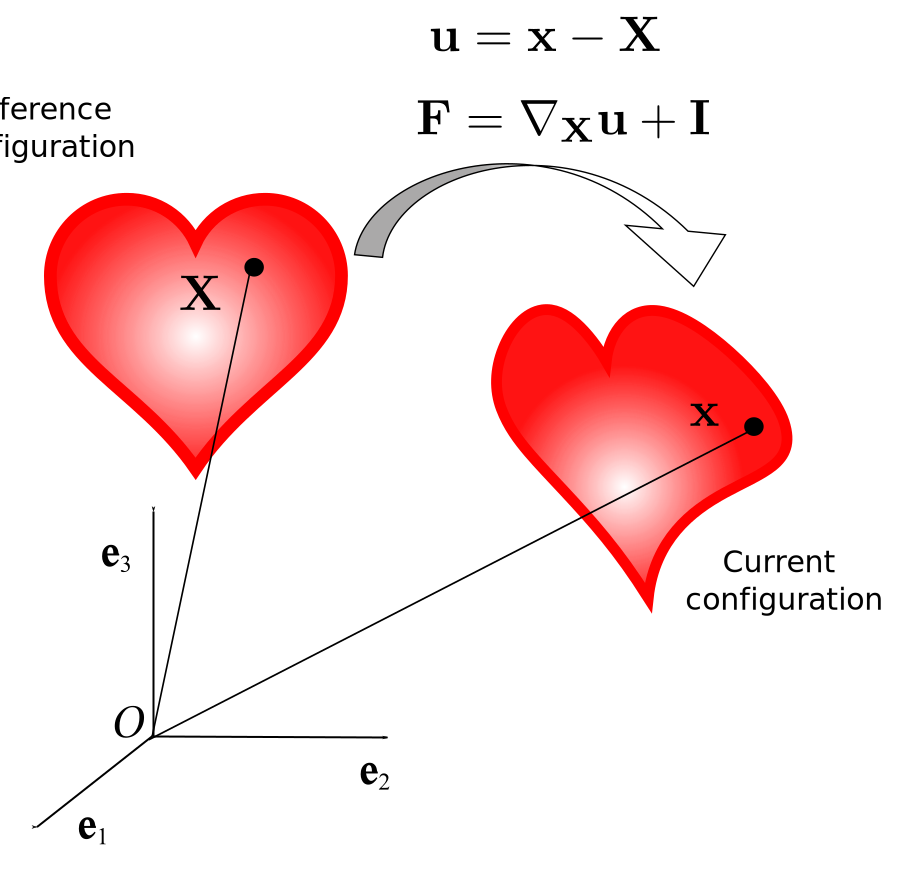
\includegraphics[width=0.6\textwidth]{chapters/introduction/figures/motion.pdf}
\caption{Relations between the current and reference configuration.}
\label{fig:motion}
\end{figure}
Some other useful quantities are the \emph{right Cauchy-Green} deformation
tensor $\C = \F^T\F$, the \emph{left Cauchy-Green} deformation tensor
$\mathbf{B} = \F\F^T$, the \emph{Green-Lagrange} strain tensor
$\mathbf{E} = \frac{1}{2}(\C - \I)$, and the determinant of the
deformation gradient $J = \det \F$.

An important concept in mechanics is the concept of stress, which is
defined as force per area
$\left[\frac{\mathrm{N}}{\mathrm{m}^2}\right]$. When working with
different configurations one needs to be careful with which forces and
which areas we are talking about. Table \ref{tab:stress_tensor}
shows how forces and areas are related for the most important stress
tensors used in this thesis. Note that the explicit form of the stress
tensor requires a constitutive law for the material at hand. This will
be discussed in more detail in Section \ref{sec:constitutive_relations}.

\begin{table}[h]
  \centering
  \begin{tabular}{lll}
    \toprule
    Stress tensor & Forces & Area \\
    \midrule
    Second Piola-Kirchhoff ($\SPK$) & Reference configuration & Reference configuration \\
    First Piola-Kirchhoff ($\FPK$) & Current configuration  &  Reference configuration \\
    Cauchy ($\Cauchy$) &  Current configuration & Current configuration  \\
    \bottomrule
  \end{tabular}
  \caption{\label{tab:stress_tensor}Showing different stress tensors
    used in this thesis, and how
    they relate forces to areas trough different configurations.}
\end{table}


\subsection{Balance laws and transformations}
In this section we will cover some basic transformations used to
derive the fore-balance equations for the mechanics of the heart. 

\subsubsection{Transformations between reference and current
  configuration}
By definition, the reference configuration $\Omega$, and current
configuration $\omega$, are related via the motion $\varphi$ in the
sense that a point $\mathfrak{p} \in \mathfrak{B}$ with reference
coordinates $\Xvec$ and current coordinates $\xvec$ satisfies $\xvec =
\varphi(\Xvec)$. Likewise a vector in the reference configuration is
related to a vector in the current configuration  via the
deformation gradient $\F$; if $\mathrm{d}\Xvec$ is a vector in the
reference configuration it will transform to the vector
$\mathrm{d}\xvec$ in the current configuration, and $\mathrm{d}\xvec =
\F \mathrm{d}\Xvec$. From this relation we also derive that the
transformation of an infinitesimal volume element in the reference
configuration, $\mathrm{d}V$ is related to an infinitesimal volume
element in the current configuration, $\mathrm{d}v$  via the determinant of the
deformation gradient,
\begin{align}
  \mathrm{d}v =\det(\F) \mathrm{d}V.
  \label{eq:volume_element}
\end{align}
Another important transformation is the transformation of normal
vectors. By noting that we can write \eqref{eq:volume_element} using
surface elements
\begin{align*}
  \mathrm{d}s \mathbf{n} \mathrm{d}\xvec  &= \mathrm{d}v = \det(\F) \mathrm{d}V = \det(\F) \mathrm{d}S  \Nvec \mathrm{d}\Xvec\\
  &\implies \left( \mathrm{d}s \mathbf{n} \F  - \mathrm{d}S \det(\F) \Nvec \right) \mathrm{d}\Xvec = 0\\
  &\implies \left( \mathrm{d}s \F^T \mathbf{n}  - \mathrm{d}S \det(\F) \Nvec \right) \mathrm{d}\Xvec = 0,\\
\end{align*}
we get \emph{Nanson's formula}
\begin{align}
  \mathrm{d}s \mathbf{n}  =  \det(\F) \F^{-T} \mathrm{d}S \Nvec,
\end{align}
which relates the normal vector in the current configuration to the
normal vector in the reference configuration.


\subsubsection{Conservation of linear momentum}
Newton's seconds law states that the change in linear momentum equals
the net impulse acting on it. For a continuum material with constant
mass density $\rho$ this implies that
\begin{align}
  \int_{\omega} \rho \dot{\mathbf{v}} \mathrm{d}v = \mathbf{f},
  && \mathbf{f} = \int_{\partial \omega} \mathbf{t} \mathrm{d}s
     + \int_{\omega} \mathbf{b} \mathrm{d}v,
     \label{eq:cons_lin_mom}
\end{align}
where $\mathbf{v}$ is the spatial velocity field, $\mathbf{t}$ is
the traction acting on the boundary, and $\mathbf{b}$ is the body
force. From \emph{Cauchy's stress theorem} we know that there exists a
second order tensor $\sigma$, known as the Cauchy stress tensor that is
related to the traction vector by $\mathbf{t} = \sigma \mathbf{n}$,
where $\mathbf{n}$ is the unit normal in the current configuration.
Using the divergence theorem we get
\begin{align*}
  \int_{\partial \omega} \mathbf{t} \mathrm{d}s
  = \int_{\partial \omega} \sigma \mathbf{n} \mathrm{d}s
  = \int_{\omega} \nabla \cdot \sigma \mathrm{d}v,
\end{align*}
and by collecting the terms from \eqref{eq:cons_lin_mom} we arrive at
Cauchy's momentum equation
\begin{align}
  \nabla \cdot \sigma + \mathbf{b} =  \rho \dot{\mathbf{v}}.
  \label{eq:chauch_momentum_eq}
\end{align}
The contribution from the body force ($\mathbf{b}$)  and inertial term
($\rho \dot{\mathbf{v}}$) can be considered negligible compared to the stresses
\cite{hunter1996kd,tallarida1970left, moskowitz1981effects}, which is
why the force balance equations is typically only stated as
\begin{align}
  \nabla \cdot \sigma = \mathbf{0}.
  \label{eq:momentum_simple_current}
\end{align}
Note that we have formulated the balance law in the current
configuration. An equivalent statement can be formulated in terms of
the reference configuration
\begin{align}
  \nabla \cdot \FPK = \mathbf{0}, 
  \label{eq:momentum_simple_reference}
\end{align}
where $\FPK$ is the first Piola-Kirchhoff stress tensor.

\subsubsection{Conservation of angular momentum}
Just like linear momentum, the angular momentum is also a conserved
quantity. We will not go through the derivation, but state that as a
consequence, the Cauchy stress tensor is symmetric
\begin{align}
  \sigma = \sigma^T.
\end{align}



\subsection{Hyperelasticity}
\label{sec:hyperelasticity}

Even though experimental studies have indicated visco-elastic behavior
of the myocardium \cite{dokos2002shear, gultekin2016orthotropic}, a
common assumption is to consider quasi-static behavior, meaning that
the inertial term in \eqref{eq:chauch_momentum_eq} is negligible and
static equilibrium is achieved at all points in the cardiac cycle. Therefore
it is also possible to model the myocardium as a hyperelastic
material,which is a type of elastic material. 
This means that we postulate the existence of
a strain-energy density function $\Psi:\mathrm{Lin}^+ \rightarrow
\mathbb{R}^+$, and that stress is given by the relation
\begin{align}
\FPK = \frac{\partial \Psi(\F)}{\partial \F}.
\end{align}
Since stress has unit Pa, we see that the strain-energy density
function is defined as energy per unit reference volume, and has units
$\frac{\text{Joule}}{m^3}$. 
The strain-energy density function relates  the amount of
energy that is stored within the material in response to a given
strain. Hence, the stresses in a hyperelastic material with a given
strain-energy density function, depend only on the strain, and not the
path for which the material deforms. On the contrary, if the model had
been visco-elastic we would expect to see hysteresis in the
stress/strain curve, but this is not possible for a hyperelastic
material. 

\begin{remark}
  The second law of thermodynamics states that the total entropy
  production in a thermodynamic process can never be negative. Elastic
  materials define a special class of materials in which the entropy
  production is zero. Within this thermodynamic framework the
  strain-energy density function coincides (up to a constant) with the
  Helmholtz free energy density.
\end{remark}


\subsubsection{General requirements for the strain-energy density
  function}
\label{sec:strain_energy_req}
Some general requirements must hold for the strain-energy function.
First of all, we require that the reference state is stress free and
that the stored energy increases monotonically with the deformation. 
Formally this can be stated simply as 
\begin{align*}
  \Psi(\I) = 0 \; && \text{and} &&\; \Psi(\F) \geq 0.
\end{align*}
Moreover, expanding or compressing a body to zero volume would
require an infinite amount of energy, i.e
\begin{align*}
  \Psi(\F) \rightarrow \infty \; && \text{as} &&\; \det \F \rightarrow& 0 \\
  \Psi(\F) \rightarrow \infty \; && \text{as} &&\; \det \F \rightarrow& \infty
\end{align*}
We say that the strain energy should be objective, meaning that the
stored energy in the material should be invariant with respect to
change of observer. Formally we must have: \emph{given any positive symmetric
rank-2 tensor $\C \in \mathrm{Sym}$:}
\begin{align}
  \Psi(\mathbf{C}) = \Psi(\mathbf{Q}\mathbf{C}\mathbf{Q}^T), \; \forall \mathbf{Q} \in \mathcal{G} \subseteq \mathrm{Orth}.
\end{align}
Here $\mathrm{Orth}$ is the group of all positive orthogonal matrices.
If $\mathcal{G} = \mathrm{Orth}$ we say that the material is
isotropic, and otherwise we say that the material is anisotropic.
This brings us to another important issue, which is related to the
choice of coordinate-system. Having to deal with different
coordinate-systems, and mapping quantities from one coordinate-system
to another can results in complicated computations. Therefore it would be beneficial if we
could work with quantities which do not depend on the choice of
coordinate-system. Such quantities are called invariants. 
If the material is isotropic, the representation theorem for
invariants states that $\Psi$ can be expressed in terms of the
principle invariants of $\mathbf{C}$, that is $\Psi = \Psi(I_1, I_2,
I_3)$. The principle invariants $I_i, i=1,2,3$ are the coefficients in
the characteristic polynomial of $\mathbf{C}$, and is given by 
\begin{align}
  I_1 = \tr \C,  && I_2 = \frac{1}{2}\left[ I_1^2 - \tr(\C^2)\right] && \text{and} && I_3 = \det \C.
\end{align}
In the case when the material constitutes a transversely isotropic
behavior, that is, the material has a preferred direction $\mathbf{a}_0$,
which in the case of the myocardium could be the direction of fiber
muscle fibers, we have
\begin{align*}
  \mathcal{G} = \{ \mathbf{Q} \in \mathrm{Orth}: \mathbf{Q}(\mathbf{a}_0\otimes\mathbf{a}_0)\mathbf{Q}^T = \mathbf{a}_0\otimes\mathbf{a}_0 \},
\end{align*}
with $\otimes$ being the outer product. In this case the strain-energy
density function can still be expressed through invariants. However,
we need to include the so called quasi-invariants, which are defined
as stretches in the local microstructural coordinate-system. The
transversely isotropic invariants are given by
\begin{align*}
  I_{4\mathbf{a}_0 } = \mathbf{a}_0 \cdot (\C \mathbf{a}_0) && \text{and} && I_5 = \mathbf{a}_0 \cdot (\C^2 \mathbf{a}_0).
\end{align*}
The invariants do have a physical interpretation. For instance, $I_3$
is related to the volume ratio of material during deformation, while
$I_{4\mathbf{a}_0 } $ is related to the stretch along the direction
$\mathbf{a}_0 $. Indeed the \emph{stretch} ratio in the direction
$\mathbf{a}_0$ is given by $\lambda_{\mathbf{a}_0} = | \F \mathbf{a}_0
|$ and we see that $I_{4\mathbf{a}_0 }  =  \mathbf{a}_0 \cdot (\C
\mathbf{a}_0) = \F \mathbf{a}_0 \cdot (\F \mathbf{a}_0) =
\lambda_{\mathbf{a}_0}^2$. For more details about invariants see e.g
\cite{holzapfel2009constitutive,liu1982representations}.


The theory of global existence of unique solutions for elastic problems
was originally based convexity of the free energy function.
An energy function $\Psi: \mathrm{Lin}^+ \rightarrow
\mathbb{R}^+$ is strictly \emph{convex} if for each $\F \in
\mathrm{Lin}^+$ and $\mathbf{H} \neq \mathbf{0}$ with $\det (\F +
(1-\lambda)\mathbf{H}) > 0$, we have
\begin{align}
  \Psi(\lambda \F + (1-\lambda) \mathbf{H})
  < \lambda \Psi(\F)
  + (1-\lambda) \Psi(\F + \mathbf{H}), && \lambda \in (0,1).
\label{eq:strain_convex}
\end{align}
If the response $\FPK$ is differentiable, then condition
\eqref{eq:strain_convex} is equivalent of saying that the response is
positive definite, 
\begin{align}
  \mathbf{H} : \frac{\partial \FPK}{\partial \F} : \mathbf{H} > 0,
  && \F \in
     \mathrm{Lin}^+, \mathbf{H} \neq \mathbf{0}.
\label{eq:response_posdev}
\end{align}

However, from a physical point of view this requirement is too strict
\cite{ball1976convexity}. A slightly weaker requirement is the strong
ellipticity condition which states that \eqref{eq:response_posdev}
should hold for any $\mathbf{H}$ of rank-one, and is analogous to
say that the strain energy function is rank-one convex. 

% that the
% strain-energy function $\Psi$ is \emph{polyconvex}, meaning that there exist
% a convex function $\phi$ such that
% \begin{align*}
%   \Psi(\F) = \phi(\F, \cof \F, \det \F).
% \end{align*}
% Note however, that if $\Psi$ is convex then it is also polyconvex.


% \subsubsection{Work conjugates}


% \begin{table}[h]
%   \centering
%   \begin{tabular}{ll}
%     \toprule
%     Stress & Strain \\
%     \midrule
%     Second Piola ($\SPiola$) & Green Lagrange ($\mathbf{E}$) \\
%     First Piola ($\FPiola$) & Deformation gradient ($\mathbf{F}$) \\
%     Cauchy ($\mathbf{\sigma}$) &  Eulerian-Almansi ($\mathbf{e}$) \\
%     \bottomrule
%   \end{tabular}
%   \caption{\label{tab:work_conjugates}Work conjugate stress-strain pairs}
% \end{table}

% By conjuagate stress-strain paris we mean that the rate of mechanical
% work is given by the stress times the strain-rate. For example,
% the total work per unit volume done by the stresses from time $t_1$ to
% $t_2$ is given by
% \begin{align}
%   \mathcal{W}(t_1, t_2) &=  \int_{t_1}^{t_2} \mathbf{P} : \dot{\F} dt
%                           = \int_{t_1}^{t_2} \frac{\partial \Psi (\F)}{\partial \mathbf{F}}  : \dot{\F} - p \F^{-T} :  \dot{\F}  dt \\
%                         &= \int_{t_1}^{t_2} \frac{D \Psi (\F)}{D t} - p\cdot 0 dt
%                           = \Psi(\F(t_2)) - \Psi(\F(t_1)).
% \end{align}
% Note that this is a measure of work per unit volume.


\subsection{Incompressibility}
\label{sec:incompressibility}

The myocardium contains small blood vessels that supply the
myocardial cells with oxygen. When the myocardium contracts, this
perfused blood is squeezed out, resulting in an overall loss of
2-4\% volume\cite{yin1996compressibility}. A material that change its
volume in response to applied loads are referred to as compressible. When the 
volume is preserved we refer to the material as incompressible.
Since 2-4\% is very little, a common assumption in cardiac mechanical modeling,
which has also been made in the work conducted in this thesis, is to assume
the myocardium to be incompressible. The reason for this choice is
purely numerical.

For an incompressible material, only isochoric motions are
possible. This means that the volume of the material does not change during
any deformation, and hence we have the constraint 
\begin{align}
  J = \det(\F) = 1.
  \label{eq:incompressible_cons}
\end{align}
The constraint \eqref{eq:incompressible_cons} can be imposed by
considering the modified strain energy function
\begin{align}
  \Psi = \Psi(\F) + p(J-1),
  \label{eq:incomp_strain_energy}
\end{align}
where $p$ is a scalar which serves as a Lagrange multiplier, but which
can be identified as the hydrostatic pressure. If we differentiate
\eqref{eq:incomp_strain_energy} with respect to $\F$ we get the First
Piola-Kirchhoff stress tensor for an incompressible material
\begin{align}
  \FPK = \frac{\partial \Psi(\F)}{\partial \F} + J p \F^{-T}.
\end{align}
Likewise the Cauchy stress tensor is given by
\begin{align}
  \Cauchy = J^{-1} \frac{\partial \Psi(\F)}{\partial \F}\F^{T} + p \I.
  \label{eq:cauchy_incomp}
\end{align}


\begin{remark}
  The sign of $p$ is determined by whether you add or subtract the term
  $ p(J-1)$ to the total strain energy in
  \eqref{eq:incomp_strain_energy}. For all practical purposes, it
  does not matter if you add or subtract the term as long as you are
  consistent. 
\end{remark}


\subsubsection{Uncoupling of volumetric and isochoric response}
The total strain energy function in \eqref{eq:incomp_strain_energy}
can be written as a sum of isochoric and volumetric components. Let
\begin{align}
  \F =  \F_{\mathrm{vol}} \F_{\mathrm{iso}},
\end{align}
then $ \F_{\mathrm{vol}} =
J^{1/3}\I$ and $\F_{\mathrm{iso}} = J^{-1/3}\F$. For
compressible materials (i.e with $J \neq 1$) it is important to consider
only deviatoric strains in the strain-energy density function, so that
$\Psi = \Psi_{\mathrm{iso}}(\F_{\mathrm{iso}}) +
\Psi_{\mathrm{vol}}(J)$. For incompressible material ($J = 1$), we
have $\F_{\mathrm{vol}} = \I$ so that such a decomposition seems
unnecessary. However, a similar decomposition has shown to be
numerically beneficial \cite{weiss1996finite}. Note that, in this case, a similar
decoupling of the stress tensors has to be done.

\subsection{Boundary Conditions}
\label{sec:mech_boudary}


Choosing the correct boundary conditions for the model is essential,
and the choice should mimic what is observed in reality. To
physiologically constrain the ventricle in a correct way is difficult,
and different approaches has been proposed.
The boundary condition at the endocardium is typically modeled as a
Neumann boundary condition, representing the endocardial blood
pressure. For the left ventricle we have
\begin{align}
  \sigma \mathbf{n} = -p_{\mathrm{lv}} \mathbf{n}, \;  \xvec \in  \lVendoCur, 
\end{align}
and for the right ventricle, ``lv'' is substituted with ``rv''.
This condition has a negative sign because the unit normal
$\mathbf{N}$ is pointing out of the domain, while the pressure is
acting into the domain. 
Note that this condition is imposed on the current configuration, and
to utilize the Lagrangian formulation we can pull back this condition
to the reference configuration to obtain
\begin{align}
  \FPK\mathbf{N} &= -p_{\mathrm{lv}} J\mathbf{F}^{-T} \cdot \mathbf{N}, \;  \Xvec \in \lVendo
\end{align}
Likewise, it is common to enforce a
Neumann boundary condition on the epicardium,
\begin{align}
\FPK\mathbf{N}  &= -p_{\mathrm{epi}}  J\mathbf{F}^{-T} \cdot \mathbf{N}, \;  \Xvec \in \epi.
\end{align}
However, the pressure $p_{\mathrm{epi}}$ is often set to zero as a
simplification. 

There exist a variety of boundary conditions at the base.
It is common to constrain the longitudinal motion of
base, even though it is observed in cardiac images that the apex tend
to be more fixed than the base. A recent study shows that taking into
account the base movement is important to capture the correct
geometrical shape \cite{palit2016passive}. However, this has not been
done in the studies in this thesis.
Fixing the longitudinal motion at the base is enforced through a
Dirichlet boundary condition,
\begin{align}
  u_1 = 0,  \;  \Xvec \in \lvbase,
\end{align}
where $u_1$ is the longitudinal component of the displacement $\uvec =
(u_1, u_2, u_3)$. To apply this type of condition, it is easiest if
the base is flat and located at a prescribed location, for example in
the $x= 0$ plane. Constraining the longitudinal motion of the base
alone is not enough since the ventricle is free to move in the basal
plane. In order to anchor the geometry it is possible to fix the
movement of the base in all directions
\begin{align}
  \uvec = \mathbf{0},  \;  \Xvec \in \lvbase,
\end{align}
or fixing the endocardial or epicardial ring
\begin{align}
  \uvec &= \mathbf{0},  \;  \Xvec \in \Gamma_{\mathrm{endo}} \\
  \uvec &= \mathbf{0},  \;  \Xvec \in \Gamma_{\mathrm{epi}}.
\end{align}

Another approach which is used in this thesis is to impose a Robin
type boundary condition at the base
\begin{align}
  \FPK \Nvec + k \uvec = \mathbf{0},  \;  \Xvec \in \lvbase, 
\end{align}
or at the epicardium to mimic the pericardium
\begin{align}
  \FPK \Nvec + k \uvec = \mathbf{0},  \;  \Xvec \in \lvepi.
\end{align}
Here $k$ can be seen as the stiffness of a spring that limits the
movement. The limiting cases, $k = 0$ and $k \rightarrow
\infty$ represent free and fixed boundary respectively.
More complex boundary conditions to mimic the pericardium are also
possible \cite{fritz2014simulation}, but not considered in this thesis.
An overview of the location of the different boundaries for the
bi-ventricular geometry is illustrated in Figure \ref{fig:boundaries}.

\begin{figure}[htbp]
  \centering
    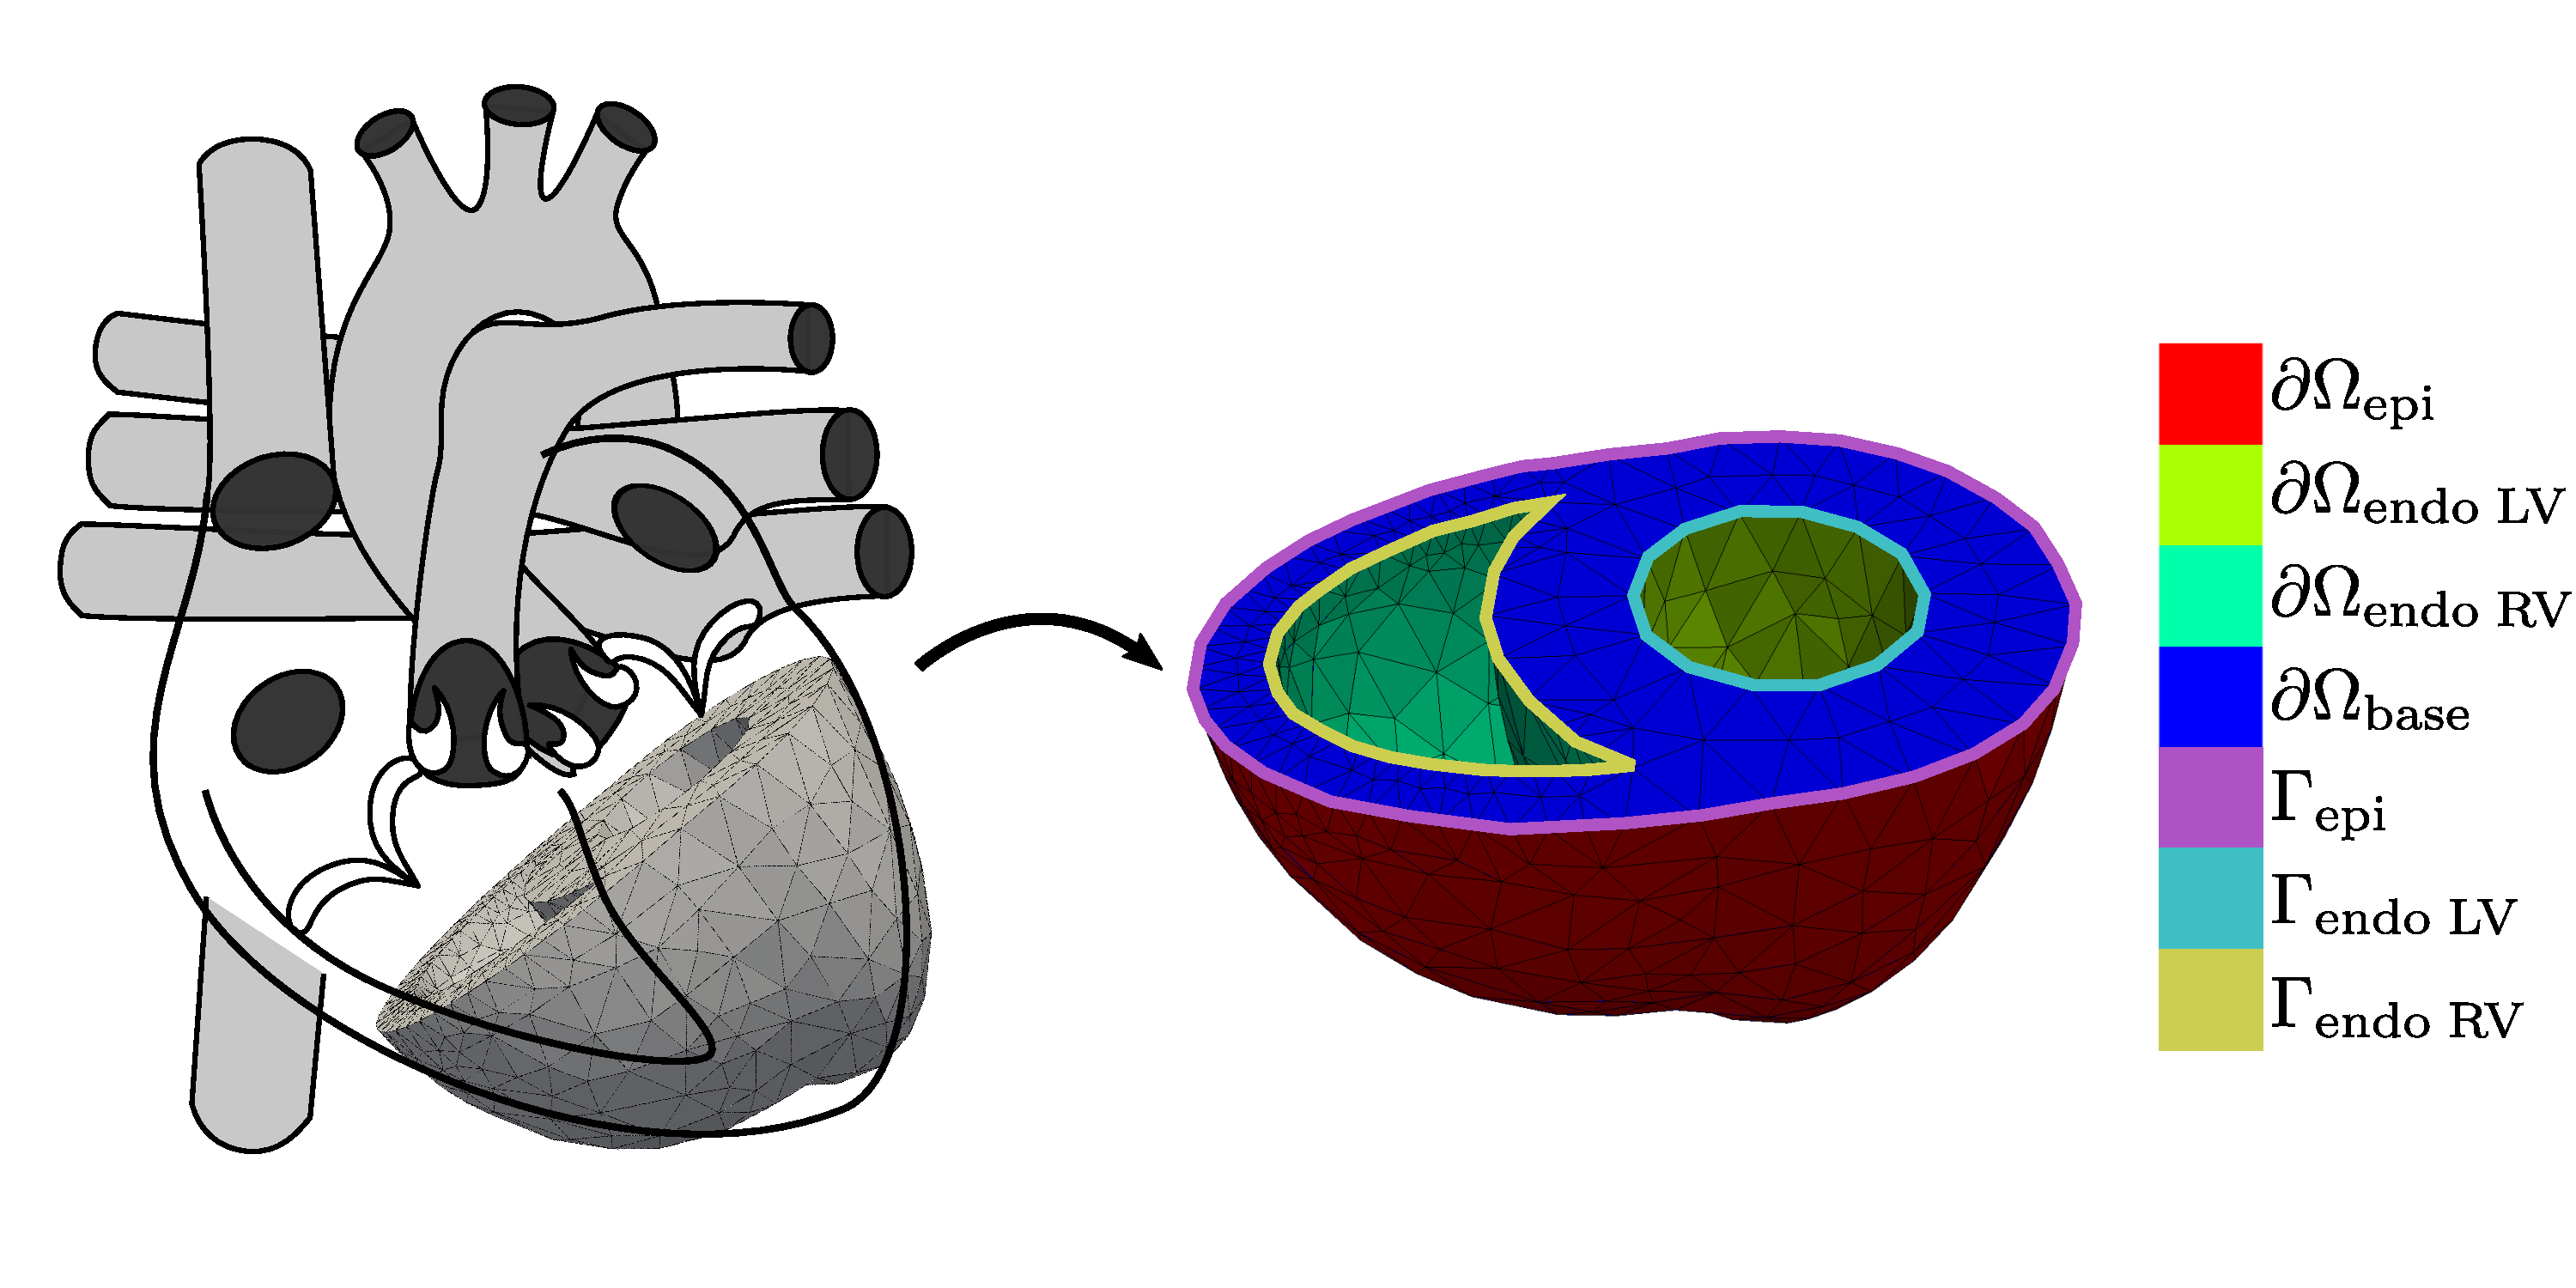
\includegraphics[width=\textwidth]{chapters/introduction/figures/boundaries}
\caption{Illustration of the different boundaries in a bi-ventricular
  domain.}
\label{fig:boundaries}
\end{figure}


\subsection{Force-balance equation}
We will now collect all the terms that are involved in the force balance for
the cardiac mechanics problem. Considering the myocardium as an incompressible,
hyperelastic material we obtain the following strong form in the
Lagrangian formulation 
\begin{align}
  \begin{split}
  \nabla \cdot \FPK &= 0 \\
  J - 1 &= 0,
  \end{split}
 \label{eq:force_balance_strong}
\end{align}
completed with appropriate boundary conditions. To solve this
numerically using the finite element method, we need to derive weak
variational form of this equation.
% \begin{align}
%   \FPK \Nvec + k \uvec &= \mathbf{0},  \;  \Xvec \in \lvbase\\
%   u_1 &= 0,  \;  \Xvec \in \lvbase \\
%   \FPK\mathbf{N}  &= \mathbf{0}, \;  \Xvec \in \epi \\
%   \FPK\mathbf{N} &= -p_{\mathrm{lv}} J\mathbf{F}^{-T} \cdot \mathbf{N}, \;  \Xvec \in \lvendo
%   \label{eq:bndry_conditions_strong}
% \end{align}
 


\subsubsection{Variational formulation}
\label{sec:variational_formulation}
There are many ways to arrive at the variational formulation of the
force-balance equations for the cardiac mechanics problem.  One way is
to consider the strong form in \eqref{eq:force_balance_strong} and use
the standard approach in the finite element method to multiply by
test function in a suitable space, and perform integration by
parts. Within the fields of continuum mechanics it is common to
refer to this approach as the \emph{principle of virtual work}, which states
that the virtual work of all forces applied to a mechanical system
vanishes in equilibrium. Within this framework, test functions are
referred to as virtual variations.
Another approach, which we will use here, derives the variational form
by utilizing a fundamental principle in physics
called the \emph{principle of stationary potential energy}, or
\emph{minimum total potential energy principle}. This principle states that a
physical system is at equilibrium when the total potential energy is
minimized, and any infinitesimal changes from this state should not add
any energy to the system.
In order to make use of this principle we first need to sum up all the
potential energy in the system. Here we separate between internal and
external energy. Internal energy is energy that is stored within the
material, for instance when you stretch a rubber band you increase its
internal energy. External energy represent the contribution from all
external forces such as gravity and traction forces.
% We consider the equilibrium in the referece domain, and denote the
% domain of interest by $\Omega \subset \mathbb{R}^3$, with boundary
% $\partial \Omega$. For the case of a left ventrcular domain we have
% $\partial \Omega = \lvendo \cup \lvepi \cup \lvbase$ and for a
% bi-ventricular domain we include $\rvendo$ in the partition as well. 
For an incompressible, hyperelastic material the total potential
energy in the system is given by
\begin{align}
  \Pi(\uvec, p) &= \Pi_{\mathrm{int}}(\mathbf{u},p) + \Pi_{\mathrm{ext}}(\mathbf{u}). \\
  \Pi_{\mathrm{int}}(\uvec,p) &= \int_{\Omega} \left[ p(J - 1) +  \Psi(\mathbf{F}) \right] \mathrm{d}V\\
  \Pi_{\mathrm{ext}}(\mathbf{u}) &= - \int_{\Omega} \mathbf{B} \cdot \mathbf{u} \mathrm{d} V - \int_{\partial \Omega_N} \mathbf{T} \cdot \mathbf{u} \mathrm{d}S
\end{align}
Here $\mathbf{B}$ represents body forces acting on a volume element in
the reference domain, e.g  gravity, and $\mathbf{T} = \mathbf{P}
\mathbf{N}$ represents first Piola-Kirchhoff traction force acting on
the Neumann boundary $\partial \Omega_N$. According to the
\emph{Principle of stationary potential energy} we have  
\begin{align}
  D_{\delta \mathbf{u}} \Pi(\mathbf{u}, p) = 0,  && \text{and} && D_{\delta p} \Pi(\mathbf{u}, p) = 0.
  \label{eq:minimum_potential_energy}
\end{align}
Here $\delta \mathbf{u}$ and $\delta p$ are virtual variations in the
space for the displacement and hydrostatic pressure respectively, and
\begin{align}
  D_{\mathbf{v}} \Phi(\mathbf{x}) = \frac{\mathrm{d}}{\mathrm{d}\varepsilon} \Phi(\mathbf{x} + \varepsilon \mathbf{v})\big|_{\varepsilon = 0}
\end{align}
is the directional derivative of $\Phi$ at $\mathbf{x}$ is the
direction $\mathbf{v}$. This operator is also known as the G\^ateaux
operator. The virtual variations $\delta \mathbf{u}$ and $\delta p$
represents an arbitrary direction with infinitesimal magnitude. We have
\begin{align}
  0 = D_{\delta p} \Pi(\mathbf{u}, p)
  = \int_{\Omega}  \delta p(J(\mathbf{u}) - 1) \mathrm{d}V,
\end{align}
and
\begin{align*}
  \begin{split}
  0 = D_{\delta \mathbf{u}} \Pi(\mathbf{u}, p) 
  =&  \int_{\Omega}  \left[ pJ \mathbf{F}^{-T} + \mathbf{P} \right] : \Grad \delta \mathbf{u} \mathrm{d}V - \int_{\Omega} \mathbf{B} \cdot \delta \mathbf{u} \mathrm{d} V
  \end{split}
\end{align*}
Note that the traction forces are now incorporated into the stress
tensors after application of the divergence theorem. These equations
are also commonly referred to as the Euler-Lagrange equations. Here $\uvec  \in V = 
\left[H_D^1(\Omega)\right]^3$, with $H_D^1(\Omega) = \{ \mathbf{v}:
\int_{\Omega} \left[ |\mathbf{v}|^2 +  |\Grad \mathbf{v}|^2
\right]\mathrm{dV} < \infty \wedge \mathbf{v}\big|_{\partial \Omega_D}
= 0\}$ and $p \in Q = L^2(\Omega)$, with $\partial \Omega_D$
representing the Dirichlet boundary. In summary, the Euler-Lagrange
equations written in a mixed form reads : \emph{Find $(\uvec, p)\in V
  \times Q$ such that} 
\begin{align}
  \begin{pmatrix}
    D_{\delta p} \Pi(\mathbf{u}, p)\\
    D_{\delta \mathbf{u}} \Pi(\mathbf{u}, p) 
  \end{pmatrix}
  = \mathbf{0}.  && \forall \; (\delta \uvec, p) \in V \times Q.
 \label{eq:intro_variational_form}
\end{align}


\subsubsection{Discretization of the force balance equations}

Equation \eqref{eq:force_balance_strong} is only possible to solve
analytically for very simplified problems. Therefore we need to employ
numerical methods to solve the problem. One such method
is the finite element method (FEM). When using the finite element method, we often refer to such
approximation as a Galerkin approximation. This is based on
approximating the solution by linear combinations of  basis functions in a finite dimensional
subspace of the true solution. If $V$ and $Q$ are two suitable Hilbert
spaces for the displacement $\uvec$ and the hydrostatic pressure $p$
respectively, we now select some finite dimensional subspaces $V_h
\subset V$ and $Q_h \subset Q$, which are spanned by a finite number
of basis functions. 


For incompressible problems such as \eqref{eq:force_balance_strong}, we cannot choose the
approximation spaces $V_h, Q_h$ at random. A known numerical issue
that arises for such saddle-point problems is \emph{locking}, which can be
seen if the material do not deform even if forces are applied. The
problem is solved by requiring the finite element approximation to
satisfy the discrete inf-sup condition \cite{le1982existence}. There
exist several mixed elements that satisfies this condition
\cite{chapelle1993inf}. The elements used in this thesis are the
Taylor-Hood finite elements \cite{taylor1973numerical}. Let the domain of
interest be denoted by $\Omega$, and let $\mathcal{T}_h$ be a
triangulation of that domain in the sense that $\bigcup_{T \in
  \mathcal{T}_h} T = \overline{\Omega}$. Let $\mathcal{P}_k
(T)$ be the linear space of all polynomials of degree $\leq k$ defined
on $T$. Then for $k \geq 2$, the Taylor-Hood finite element spaces are the spaces
\begin{align}
  V_h = \{  \phi \in C(\Omega) \;  | \; \phi \big| T  \in \mathcal{P}_k (T) , T \in \mathcal{T}_h \},\\
  Q_h = \{  \phi \in C(\Omega) \;  | \; \phi \big| T  \in \mathcal{P}_{k-1} (T) , T \in \mathcal{T}_h \},
\end{align}
where $C(\Omega)$ denotes the space of continuous function on
$\Omega$. In this thesis we have exclusively used these elements with
$k = 2$.



\begin{remark}
  The basis functions that span the Taylor-Hood
  finite element spaces are also known as the
  Lagrangian basis functions. These basis functions, of
  degree $n$, are polynomials of degree $n$ on each element, but only
  continuous at the nodes (i.e not continuously
  differentiable). Consequently, differentiating a function that is
  expressed as a linear combination of the Lagrangian basis functions,
  will not be continuous at the nodes, and therefore caution has to
  be made when evaluating features that depends on the derivative of
  such functions. Examples of such features are stress and
  strain with depends on the deformation gradient which again depends
  on the derivative of the displacement. One way to deal with this
  issue is to 1) use other types of elements that are continuously
  differentiable everywhere,  such a the cubic Hermite elements or 2) evaluate the features at the
  Gaussian quadrature points where there is no problem with continuity.
\end{remark}


\subsection{Constitutive relations}
\label{sec:constitutive_relations}
We have now covered a mechanical framework which holds any for
material in general. What differentiate the mechanics of soft
living tissue, like the myocardium, from other materials is the
constitutive relations which describes the response of a material to
applied load. Such constitutive relations often comes from
experimental observations, both observations of anatomical structure
but also from experiments done on tissue slabs.

We have already covered the theory of hyperelasticity and incompressibility in Section
\ref{sec:hyperelasticity} and \ref{sec:incompressibility} respectively
which are types of constitutive relations. In this section we will
cover constitutive relations which only apply to soft living tissue
such as the myocardium. In particular, we will consider a complete
constitutive model of the mechanical behavior of the myocardium that
accounts for both the passive and the active response of the myocardium.


\subsubsection{Modeling of the passive myocardium}


The passive response of the myocardium has been investigated through
uni-axial, bi-axial and shear deformation experiments \cite{dokos2002shear}.
% Look at Humprey Continuum biomechanics of
% soft biological tissues
In 2009 Holzapfel and Ogden proposed an orthotropic constitutive model
of the passive myocardium \cite{holzapfel2009constitutive} which is
based on the experiments done in \cite{dokos2002shear}, and is the
model used in this thesis. Other constitutive models for the passive
myocardium exists
\cite{costa2001modelling,guccione1991passive,nash2000computational}
but is not considered here. The model
assumes a local orthonormal coordinate system with the fiber axis
$\ef$, sheet axis $\eS$ and sheet-normal axis $\en$. %The subscript
% refers that the vectors $(\ef, \eS, \en)$ are vectors in the reference
% configuration.
From this coordinate system we define the invariants
\begin{align}
  \begin{split}
    I_1 &= \tr(\C) ,\\
    I_{4\ef} &= \ef \cdot (\C \ef),\\
    I_{4\eS} &= \eS \cdot (\C \eS),\\
    I_{8\ef\eS} &=  \eS \cdot (\C \ef), 
  \end{split}
\end{align}
Here $I_{4\ef} $ and $I_{4\eS}$ are the stretches along the
fiber, sheet axis respectively and $I_{8\ef\eS}$ is
related to the angle between the fiber and sheets in the current
configuration given that they are orthogonal in the reference
configuration. Note that since $(\ef, \eS, \en)$ is an orthonormal
system, we have the relation $I_1 = I_{4\ef} + I_{4\eS} +I_{4\en}$,
and so $I_{4\en}$ is redundant. The orthotropic Holzapfel and Ogden
model reads
\begin{align}
  \label{eq:holzapel_full}
  \begin{split}
  \Psi(I_1, I_{4\ef},  I_{4\eS},  I_{8\ef\eS}) =& \frac{a}{2 b} \left( e^{ b (I_1 - 3)}  -1 \right)\\
  +& \frac{a_f}{2 b_f} \left( e^{ b_f (I_{4\ef} - 1)_+^2} -1 \right) \\
  +& \frac{a_s}{2 b_s} \left( e^{ b_s (I_{4\eS} - 1)_+^2} -1 \right)\\
  +& \frac{a_{fs}}{2 b_{fs}} \left( e^{ b_{fs} I_{8\ef\eS}^2} -1 \right).
\end{split}
\end{align}
Here $( x )_+ = \frac{1}{2} \left( x + |x| \right)$, so that the
the terms involving $I_{4\ef}$ and $I_{4\eS}$ only contribute to the
stored energy during elongation. From \eqref{eq:holzapel_full} we see
that it is easy to identify the physical meaning of each term. For
example the first term represents the isotropic contribution which is
the overall stiffness in the extracellular matrix while the second
term accounts for the extra stiffness along the fibers when they are
elongated. It is also straight forward to prove that the strain-energy
function is convex, and that the requirements for existence and
uniqueness discussed in Section \ref{sec:strain_energy_req} are
fulfilled.

In this thesis we have in used a transversely isotropic version of
\eqref{eq:holzapel_full} which is obtained by setting $a_{fs} =
b_{fs}= a_s = b_s = 0$, i.e 
\begin{align}
  \label{eq:holzapel_trans}
  \begin{split}
  \Psi(I_1, I_{4\ef}) = \frac{a}{2 b} \left( e^{ b (I_1 - 3)}  -1 \right)
  + \frac{a_f}{2 b_f} \left( e^{ b_f (I_{4\ef} - 1)_+^2} -1 \right).
  \end{split}
\end{align}
If we further set $a_f = b_f = b = 0$ so that in $a$ is the
only nonzero parameter, then the Holzapfel-Ogden model reduces (after a
series expansion of the exponential and a limiting argument) to
\begin{align}
  \Psi(I_1)  = \frac{a}{2} \left( I_1 - 3 \right), 
\end{align}
which is the model of a Neo Hookean material. The Cauchy stress can be derived
analytically from \eqref{eq:holzapel_full}, by using the chain rule and
\eqref{eq:cauchy_incomp}, 
\begin{align}
  \begin{split}
    J\Cauchy
    =& \frac{\partial \Psi(\F)}{\partial \F}\F^{T} + p \I
    = \sum_{i \in \left\{ 1, 4\ef,  4\eS,  8\ef\eS \right\} }
    \psi_i \frac{\partial I_i}{\partial \F}\F^{T} + p \I \\
    =& p \I + a \left( e^{ b (I_1 - 3)}  -1 \right) \mathbf{B} 
    + 2 a_f (I_{4\ef} - 1)_+  e^{ b_f (I_{4\ef} - 1)^2} \mathbf{f} \otimes \mathbf{f} \\
    &+ 2 a_f (I_{4\eS} - 1)_+  e^{ b_f (I_{4\eS} - 1)^2} \mathbf{s} \otimes \mathbf{s} 
    + a_{fs} I_{8\ef\eS}  e^{ b_{fs} I_{8\ef\eS}^2} \left( \mathbf{f} \otimes \mathbf{s}  +  \mathbf{s} \otimes \mathbf{f} \right),
  \end{split}
\end{align}
where $\mathbf{B} = \F \F^{T}$ is the left Cauchy-Green tensor,
$\mathbf{f} = \F \ef$ and $\mathbf{s} = \F \eS$.

\subsubsection{Modeling of the active contraction}
  

One feature that separates the myocardium from other hyperelastic
materials such as rubber, is its ability to actively generate force
without external loads. This active component of the model can be
incorporated using two fundamentally different approaches known as the
\emph{active stress} and \emph{active strain} formulation.


% As discussed 
% in Section \ref{sec:ventricular_pumping_function}, the myocardium
% contracts in a cyclic manner. 

% There are basically two main approaches to model the active response
% of the myocardium; the \emph{active stress} and the \emph{active strain}
% formulation.

\begin{figure}[htbp]
  \centering
    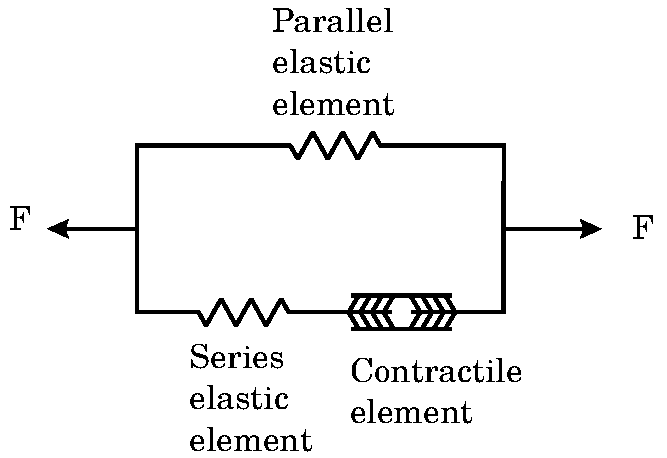
\includegraphics[width=0.5\textwidth]{chapters/introduction/figures/Hill_muscle_model.pdf}
\caption{The classical three-element Hill muscle model with one
  contractile element and two non-linear springs, one arranged in
  series and one parallel. }
\label{fig:hill_muscle_model}
\end{figure}



The \emph{active stress} approach is based on the classical three element
Hill model illustrated in Figure \ref{fig:hill_muscle_model}, where the
active contribution naturally decomposes the total stress into a sum
of passive and active stresses
\cite{nash2004electromechanical}. Hence, in the active stress
formulation \cite{hunter1998modelling} one assumes that the total
Cauchy stress $\Cauchy$ can be written as an additive sum of one
passive contribution $\Cauchy_p$ and one active contribution $\Cauchy_a$,
\begin{align}
  \Cauchy = \Cauchy_p + \Cauchy_a
\end{align}
The passive contribution is determined by the material model used
\begin{align}
 \Cauchy_p = \frac{1}{J} \frac{\partial \Psi(\F)}{\partial \F} \F^{T},
\end{align}
while the active contribution is given by 
\begin{align}
  \Cauchy_a = \Cauchy_{ff} \Fef \otimes \Fef +
  \Cauchy_{ss} \mathbf{s} \otimes \mathbf{s} +
  \Cauchy_{nn} \mathbf{n} \otimes \mathbf{n},
\end{align}
and the different constants $\Cauchy_{ff}, \Cauchy_{ss}$, and
$\Cauchy_{nn}$, which are the active stress in the fiber, sheet and
sheet-normal direction respectively, are typically coupled to the
electrophysiology and calcium dynamics.
There are experimental evidence that the active stresses in the
transverse direction of the fibers ($\Cauchy_{ss}$, and $\Cauchy_{nn}$),
are non-negligible \cite{lin1998multiaxial}, and one approach is to assume
a uniform transverse activation in which the total active tension
can be written as 
\begin{align}
  \Cauchy_a = T_a \left[\Fef \otimes \Fef +
   \eta\left( \mathbf{s} \otimes \mathbf{s} +
  \ \mathbf{n} \otimes \mathbf{n} \right)\right],
  \label{eq:intro_active_stress}
\end{align}
where $\eta$ represent the amount of transverse activation and $T_a
\in \mathbb{R}$ is the magnitude of the active tension.
In the limiting case ($\eta = 0.0$), the active tension acts purely
along the fibers and \eqref{eq:intro_active_stress} reduces to 
\begin{align}
  \Cauchy_a = T_a \Fef \otimes \Fef.
\end{align}
Note that, by observing  that
\begin{align*}
  \frac{\partial I_{4\mathbf{a}_0}}{\partial \F}
  = \frac{\partial (\mathbf{a}_0  \cdot \C \mathbf{a}_0 )}{\partial \F}
  = 2 \mathbf{a} \otimes \mathbf{a}_0 \implies
  \mathbf{a} \otimes  \mathbf{a}= \frac{1}{2} \frac{\partial I_{4\mathbf{a}_0}}{\partial \F} \F^{T}
\end{align*}
and that $I_1 =  I_{4\ef} +  I_{4\eS} +  I_{4\en}$, 
we can instead decompose the strain-energy function into a passive and active
parts \cite{pathmanathan2010cardiac}, $\Psi= \Psi_p + \Psi_a$, with
\begin{align}
\Psi_a = \frac{T_a}{2J} \left(( I_{4\ef} - 1)  + \eta \left[ (I_1 - 3) -
    (I_{4\ef} - 1)\right] \right), 
\end{align}
so that $J \Cauchy_a  = \frac{\partial \Psi_a}{\partial \F}
\F^{T}$.

The \emph{active strain} formulation is a relatively new way of modeling the
active contraction in the heart and was first introduced in
\cite{taber2000modeling}. This formulation is based on a
multiplicative decomposition of the deformation gradient, 
\begin{equation}
 \F = \F_e \F_a.
\label{eq:active_strain}
\end{equation}


The active part $\F_a$, is an inelastic process driven by the
biochemistry and can be seen as the actual distortion of the
microstructure. The elastic part $\F_e$ is responsible for preserving
compatibility of the tissue and stores all the energy in the
deformations. As a consequence, the strain energy function is a
function of the elastic deformation gradient only. The
decoupling can illustrated by considering two sarcomeres connected in
series as shown in Figure \ref{fig:actstrain}. 

\begin{figure}[htbp]
  \centering
    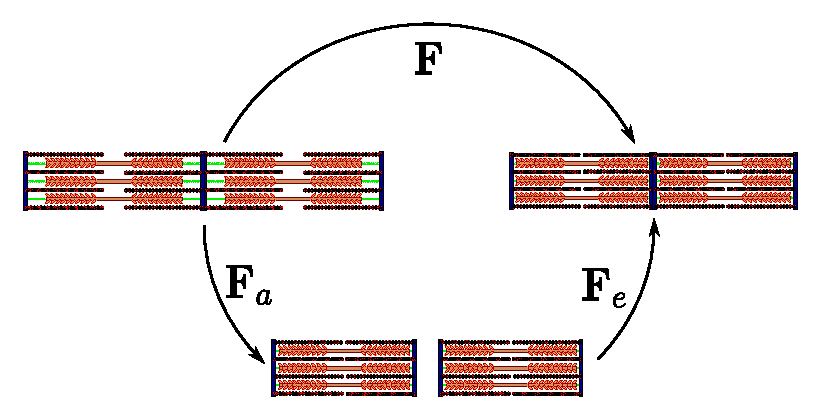
\includegraphics[width=0.7\textwidth]{chapters/introduction/figures/actstrain.pdf}
\caption{Illustration of the active strain formulation. During the active
deformation, the sarcomeres shortens as if they were all detached. The
elastic deformation ensures compatibility of the tissue.}
\label{fig:actstrain}
\end{figure}


The general form of the active deformation gradient for a
material with an orthotropic active response is given by
\begin{equation}
  \F_a =  \I
  - \gamma_f \ef \otimes \ef
  - \gamma_s \eS \otimes \eS
  - \gamma_n \en\otimes \en
 \label{eq:active_strain_Fa_general}
\end{equation}

We add the constraint $\det(\F_a) = 1$, meaning that the active
deformation is volume preserving. Further we assume that the activation is
transversely isotropic, so that the sheet and sheet-normal axis is
treated in the same way. It is then straight forward to verify that
$\gamma_n = \gamma_s =1- (1-\gamma_f)^{-1/2}$, and we have
\begin{equation}
  \F_a = (1 - \gamma) \ef \otimes \ef  + \frac{1}{\sqrt{1 - \gamma}} (\I - \ef \otimes \ef), 
 \label{eq:intro_active_strain_Fa_gjerald}
\end{equation}
where we set $\gamma = \gamma_f$ for convenience. 


While the motivation behind the active stress formulation is purely
physiological and based on the classical Hill model shown in Figure
\ref{fig:hill_muscle_model}, the motivation behind the active strain
formulation is more driven by ensuring mathematical robustness. In
particular it has been shown \cite{ambrosi2012active} that with the
active strain formulation, properties such as frame invariance and
rank-one ellipticity is inherited from the strain energy function. In
contrast, rank-one ellipticity is not guaranteed for the active stress
formulation.

For a more extensive comparison of the active stress and active strain
approach we refer to \cite{ambrosi2012active,giantesio2017comparison},
and for an overview of other methods to model the active contraction
we refer to \cite{goriely2017five}.



\subsection{Implementation details}
The cardiac mechanics solver developed during the work of this thesis
is implemented using the finite element framework FEniCS. Here we
briefly explain the main components of FEniCS as well as some
numerical considerations made when implementing the solver.


\subsubsection{The FEniCS Project}
\label{sec:fenics}

The FEniCS project is an open-source computing platform for solving
partial differential equations (PDEs) using the finite element method (FEM).
Solving PDEs using FEM involves many implementation details that can
be tedious to implement yourselves. The idea behind FEniCS is to
automate code generation so that the user can spend more time on doing
research and less time on implementation of assembly matrices. At the
core of FEniCS is DOLFIN \cite{logg2012dolfin}, which is C++/Python
library, and works as the main interface in FEniCS. In this thesis
only the Python interface has been used, in which C++ code is
automatically generated using SWIG. This allows for simplicity through
the Python scripting language and the speed of the C++ language.
The domain specific language used to represent weak formulations is
called the Unified Form Language (UFL) \cite{alnaes2014unified}, and
allows for e.g automatic differentiation of forms and expressions. The
FEniCS form compiler (FFC) \cite{logg2012ffc} compiles code written in
UFL to Unified Form-assembly Code (UFC) \cite{alnaes2012ufc} which are
optimized C++ code. The Python interface also makes use of the Instant
module which allows for just-in-time (JIT) compilation of C++
code. The compiled code is also stored in a cache so that compilation
of a form only happens once. Also, the relatively new UFL Analyser and
Compiler System (UFLACS) allows for fast compilation of complex forms
such as variational formulations that include the Holzapfel Ogden
material model \eqref{eq:holzapel_full}. 

For more information about FEniCS, the reader is referred to the
official web page (\url{https://fenicsproject.org}) or any of the
cited literature.

\subsubsection{Numerical considerations}
The solution of non-linear problems such as the one described here are
typically solved using methods like Newton's method. The convergence of
such methods depends on the initial guess, and if the
initial guess is too far from the true solution, the solver might diverge.
Moreover, if the initial guess is close to the true solution the
convergence rate is in general quadratic.

Let us consider a
typical numerical problem of inflating the ventricular geometry from a
stress-free configuration to end-diastole. This involves increasing
the pressure, or the boundary traction on the endocardium, from zero
to the end-diastolic pressure. A strategy know as the
\emph{incremental load} technique is usually a good approach. In this
strategy you select some incremental step-size (for instance $0.4$
kPa), and increase the pressure linearly until the target pressure is
reached. If the solver diverges you decrease the step-size (for
instance by a factor of 0.5) until convergence is reached, and
continue to step up the pressure with the new step-size. This is very
robust, but definitely a slow approach. Since many of the 
constitutive models for myocardium consist of an exponential
relationship between the stress and strain (so called Fung-type
relation), the amount of stress needed to displace a material will be
higher if the material is a state with high strain compared to a state
of low strain. Therefore, in the low strain state, the Newtons solver
might perform fewer iterations to reach convergence when the load is increased. As a
result, one could improve the incremental load technique by adapting
the step size if the number of newton iterations are below a certain
threshold (for instance $8$ iterations).

An even more clever strategy uses a technique from bifurcation and
chaos theory and is known as numerical continuation
\cite{allgower2003introduction}.  Suppose we want to
solve the non-linear problem $F(\uvec, \lambda)=0$ with state variable
$\uvec$ and parameter $\lambda$. For instance $\uvec$ could be the
displacement and $\lambda$ could be the endocardial pressure.
The idea behind numerical continuation is that given a solution pair
$(\uvec_0, \lambda_0)$ there exist (under conditions stated by the
implicit function theorem) a solution curve $\uvec(\lambda)$ such that
$F(\uvec(\lambda), \lambda)=0$ and $\uvec(\lambda_0) = \uvec_0$.
To explicitly find such a curve is not always easy but a simple
approximation can be found by extrapolation: Given two pairs
$(\uvec_0, \lambda_0)$ and $(\uvec_1, \lambda_1)$, and a new target
parameter $\lambda_2$, a possible solution is 
\begin{align}
  \uvec_2 =  (1-\delta)\uvec_0 + \delta \uvec_1 && \delta = \frac{\lambda_2 - \lambda_0}{\lambda_1 - \lambda_0}.
\end{align}
% Let $w_0$ denote the initial
% state variable associated with endocardial pressure $p_0$. Increase
% the pressure $p_1 = p_0 + \Delta p_0$, and solve to obtain $w_1$. Next
% we would like to solve for $p_2 = p_1 + \Delta p_1$ where $\Delta
% p_1$ might be the adapted step size. In stead of using $\tilde{w_2}=w_1$ as
% initial guess for the newton solver, as we typically would do in the incremental load
% technique, we observe that if $\delta = \frac{p_2 - p_0}{p_1 - p_0}$,
% and hence $p_2 = (1-\delta)p_0 + \delta p_1$, then a better choice
% of intial guess would be $\tilde{w_2} = (1-\delta)w_0 + \delta w_1$.
Choosing $\uvec_2$ as initial guess for the non-linear solver has been
successfully performed by others in non-linear cardiac mechanics
problems \cite{pezzuto2013mechanics}, and this approach is also used
in this thesis. 





%%% Local Variables:
%%% mode: latex
%%% TeX-master: "../../main"
%%% End: